\documentclass[12pt]{article}
\usepackage[english]{babel}
\usepackage[utf8]{inputenc}
\usepackage{amsmath, amssymb, amsthm}
\usepackage{graphicx}
\usepackage{hyperref}
\usepackage[margin=.75in]{geometry}
\usepackage{xcolor}
\usepackage{tikz}

\newtheorem{theorem}{Theorem}
\newtheorem{prop}{Proposition}
\newtheorem*{prop*}{Proposition}
\newtheorem{obs}{Observation}
\newtheorem*{obs*}{Observation}

\setlength{\topmargin}{0pt}
\setlength{\headsep}{0pt}
\textheight = 600pt

\title{Graph Theory \\ Homework 9}
\author{Ben Kallus and Nicholas Adair}
\date{Due Monday, Monday, March 15}

\begin{document}
\maketitle

\noindent{\bf 6.4}

{\bf (a)} $G = C_5$

{\bf (b)} $G = K_3$

{\bf (c)} $G = P_4$

{\bf (d)} $G = P_2$

{\bf (e)} $G:$
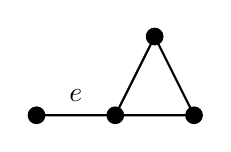
\begin{tikzpicture}
	\draw[fill=black] (0, 0) circle (3pt);
	\draw[fill=black] (1, 0) circle (3pt);
	\draw[fill=black] (2, 0) circle (3pt);
	\draw[fill=black] (1.5, 1) circle (3pt);

	\node at (.5, .25) {$e$};

	\draw[thick] (0,0) -- (1,0) -- (2,0) -- (1.5,1) -- (1,0);
\end{tikzpicture}

\newpage\noindent{\bf 6.6}

% You haven't yet shown that there are no cut-vertices. Just use the theorem about all paths between u and w and show that all non-adjacent vertices have a path through b and a path through c.
\newpage\noindent{\bf 6.10} Proposition: If $G$ is a 6-regular graph of order 10, then for all $u,v \in V(G)$, $G$, $G - u$, and $G - u - v$ are all Hamiltonian.
\begin{proof}
	Let $G$ be a 6-regular graph of order 10.
	Then, $\delta(G) = 6 \geq \frac{10}2$.
	Thus, by Corollary 6.7, $G$ is Hamiltonian.

	Let $u \in V(G)$.
	Then, because $G$ is 6-regular, $G-u$ has 6 vertices of degree 5 and 3 vertices of degree 6.
	Thus, $\delta(G-u) = 5 \geq \frac{9}2$.
	Thus, by Corollary 6.7, $G-u$ is Hamiltonian.

	Let $v \in G-u$.
	Then, since $G-u$ consists only of degree 5 and 6 vertices, and contains only 3 degree-6 vertices, $v$ must be adjacent to a vertex of degree 5 in $G-u$.
	Thus, $\delta(G - u - v) = 4 \geq \frac{8}{2}$.
	Thus, by Corollary 6.7, $G-u-v$ is Hamiltonian.
\end{proof}

\newpage\noindent{\bf 6.14}

{\bf (a)}
\begin{proof} There exists a 2-connected Eulerian graph that is not Hamiltonian.
	Consider the following graph, $G$:
	\begin{center}
	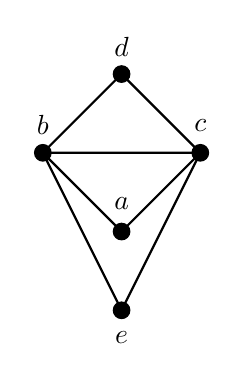
\begin{tikzpicture}
		\draw[fill=black] (0,0) circle (3pt);
		\node at (0,.35) {$b$};
		\draw[fill=black] (1,1) circle (3pt);
		\node at (1,1.35) {$d$};
		\draw[fill=black] (2,0) circle (3pt);
		\node at (2,.35) {$c$};
		\draw[fill=black] (1,-1) circle (3pt);
		\node at (1,-.65) {$a$};
		\draw[fill=black] (1,-2) circle (3pt);
		\node at (1,-2.35) {$e$};
		\draw[thick] (0,0) -- (1,1) -- (2,0) -- (1,-1) -- (0,0) -- (1,-2) -- (2,0) -- (0,0);
	\end{tikzpicture}
	\end{center}

	Clearly, by Theorem 6.1, $G$ is Eulerian.

	Suppose that $G$ were Hamiltonian.
	Then, $G$ contains a Hamiltonian cycle $C$ with first edge $ab$.\footnote{Since $b$ and $c$ are in symmetric positions, the same argument applies if the cycle starts with $ac$, instead.}
	Thus, since $a$ is incident to only two edges, $C$'s last edge must be $ca$.
	Note that $C$'s second edge must be one of $bd, be, bc$.
	Suppose that $C$'s second were $bc$.
	Then, since $C$ is a cycle with last edge $ca$, it must be that $C = (a, b, c, a)$, which is not a Hamiltonian cycle.
	Thus, $C$'s second edge cannot be $bc$.
	Now, suppose that $C$'s second edge were $bd$.
	Then, $C$'s third edge must be $dc$.
	Then, by the same logic used previously, it must be that $C = (a, b, d, c, a)$, which is not a Hamiltonian cycle.
	Since $e$ and $d$ are in symmetric positions in $G$, the same argument shows that $C$'s second edge also cannot be $be$.
	Thus, no Hamiltonian cycle exists in $G$, so $G$ is not Hamiltonian.
\end{proof}

{\bf (b)} There exists a Hamiltonian graph that is not Eulerian and has an Eulerian complement.
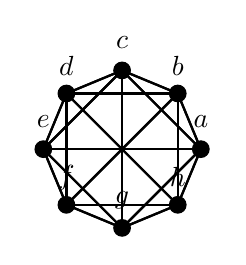
\begin{tikzpicture}
\draw[fill=black] (1.0, 0.0) circle (3pt);
\node at (1.0, 0.35) {$a$};
\draw[fill=black] (0.707, 0.707) circle (3pt);
\node at (0.707, 1.057) {$b$};
\draw[fill=black] (0.0, 1.0) circle (3pt);
\node at (0.0, 1.35) {$c$};
\draw[fill=black] (-0.707, 0.707) circle (3pt);
\node at (-0.707, 1.057) {$d$};
\draw[fill=black] (-1.0, 0.0) circle (3pt);
\node at (-1.0, 0.35) {$e$};
\draw[fill=black] (-0.707, -0.707) circle (3pt);
\node at (-0.707, -0.357) {$f$};
\draw[fill=black] (-0.0, -1.0) circle (3pt);
\node at (0.0, -0.65) {$g$};
\draw[fill=black] (0.707, -0.707) circle (3pt);
\node at (0.707, -0.357) {$h$};

\draw[thick] (1.0, 0.0) -- (-0.0, -1.0);
\draw[thick] (1.0, 0.0) -- (0.707, 0.707);
\draw[thick] (1.0, 0.0) -- (-1.0, 0.0);
\draw[thick] (1.0, 0.0) -- (0.0, 1.0);
\draw[thick] (1.0, 0.0) -- (0.707, -0.707);
\draw[thick] (0.707, 0.707) -- (1.0, 0.0);
\draw[thick] (0.707, 0.707) -- (-0.707, 0.707);
\draw[thick] (0.707, 0.707) -- (0.0, 1.0);
\draw[thick] (0.707, 0.707) -- (-0.707, -0.707);
\draw[thick] (0.707, 0.707) -- (0.707, -0.707);
\draw[thick] (0.0, 1.0) -- (-0.0, -1.0);
\draw[thick] (0.0, 1.0) -- (1.0, 0.0);
\draw[thick] (0.0, 1.0) -- (0.707, 0.707);
\draw[thick] (0.0, 1.0) -- (-1.0, 0.0);
\draw[thick] (0.0, 1.0) -- (-0.707, 0.707);
\draw[thick] (-0.707, 0.707) -- (0.707, 0.707);
\draw[thick] (-0.707, 0.707) -- (-1.0, 0.0);
\draw[thick] (-0.707, 0.707) -- (0.0, 1.0);
\draw[thick] (-0.707, 0.707) -- (-0.707, -0.707);
\draw[thick] (-0.707, 0.707) -- (0.707, -0.707);
\draw[thick] (-1.0, 0.0) -- (-0.0, -1.0);
\draw[thick] (-1.0, 0.0) -- (1.0, 0.0);
\draw[thick] (-1.0, 0.0) -- (-0.707, 0.707);
\draw[thick] (-1.0, 0.0) -- (0.0, 1.0);
\draw[thick] (-1.0, 0.0) -- (-0.707, -0.707);
\draw[thick] (-0.707, -0.707) -- (-0.0, -1.0);
\draw[thick] (-0.707, -0.707) -- (0.707, 0.707);
\draw[thick] (-0.707, -0.707) -- (-1.0, 0.0);
\draw[thick] (-0.707, -0.707) -- (-0.707, 0.707);
\draw[thick] (-0.707, -0.707) -- (0.707, -0.707);
\draw[thick] (-0.0, -1.0) -- (1.0, 0.0);
\draw[thick] (-0.0, -1.0) -- (-1.0, 0.0);
\draw[thick] (-0.0, -1.0) -- (0.0, 1.0);
\draw[thick] (-0.0, -1.0) -- (-0.707, -0.707);
\draw[thick] (-0.0, -1.0) -- (0.707, -0.707);
\draw[thick] (0.707, -0.707) -- (-0.0, -1.0);
\draw[thick] (0.707, -0.707) -- (1.0, 0.0);
\draw[thick] (0.707, -0.707) -- (0.707, 0.707);
\draw[thick] (0.707, -0.707) -- (-0.707, 0.707);
\draw[thick] (0.707, -0.707) -- (-0.707, -0.707);
\end{tikzpicture}

\newpage\noindent{\bf 6.16} Let $G$ be a connected $r$-regular graph of even order $n$ such that $\overline G$ is connected.

{\bf (a)} Proposition: Either $G$ or $\overline G$ is Eulerian.
\begin{proof}
	Suppose that neither $G$, nor $\overline G$ is Eulerian.
	Then, since $G$ is not Eulerian, by Theorem 6.1, $r$ is odd.
	Thus, $\overline G$ is $(n-1-r)$-regular.
	Since $n-1-r$ is even, $\overline G$ must be Eulerian, which contradicts our supposition.
	Thus, either $G$ or $\overline G$ is Eulerian.
\end{proof}

{\bf (b)} Proposition: Either $G$ or $\overline G$ is Hamiltonian.
\begin{proof}
	
\end{proof}


\newpage\noindent{\bf 6.20} Proposition: If $G$ is a graph of order $n \geq 3$ with the property that for each $v \in V(G)$, there is a Hamiltonian path with initial vertex $v$, then $G$ is 2-connected, and not necessarily Hamiltonian.
\begin{proof}
	Let $G$ be a graph of order $n \geq 3$ with the property that for each $v \in V(G)$, there is a Hamiltonian path with initial vertex $v$.
	Let $x, y \in V(G)$.
	Then, there exists a Hamiltonian path $P = (x = p_0, \hdots, p_i = y, \hdots, p_n)$ starting at $x$.
	Thus, $P' = (x = p_0, \hdots, p_i = y)$ is an $x-y$ path in $G$, so $G$ is connected.
	Suppose that $G$ were to have a cut-vertex $c$.
	Then, there exist $u,w \in V(G)$ with $u \neq v \neq w$ such that all $u-w$ walks contain $c$.
	Consider a Hamiltonian path $C$ with initial vertex $c$.
	Suppose, without loss of generality, that $u$ comes before $w$ in $C$.
	Consider $C'$, the subsequence of $C$ starting at $u$ and ending at $w$.
	Since $c$ is the initial vertex of $C$, it must not be present in $C'$.
	Thus, $C'$ is a $u-w$ walk that does not contain $c$, which contradicts the result that all $u-w$ walks contain $c$.
	Thus, $G$ must have no cut-vertices.
	Thus, $G$ is 2-connected.

	Observe that $G$ need not be Hamiltonian: FINISH ME
\end{proof}

\newpage\noindent{\bf 6.22}

	{\bf (a)} Yes. OBVIOUS; just disconnect the graph.

	{\bf (b)} Yes. Start with bipartite and leave a degree 1.

\newpage\noindent{\bf 6.24}



\newpage\noindent{\bf ALSO (1)}

\newpage\noindent{\bf ALSO (2)}

\end{document}
